\chapter{Corner Simulations}
Corner analysis is performed to simulate the circuit's performance against a set of parameters belonging to extreme manufacturing variations. Corner simulations are performed to verify that the circuit works at all possible conditions of process, supply voltage and temperature. Analog circuit designs that perform sufficiently well across these corners are to be considered a robust design.

\section{Process Variation}

Process variation is the naturally occurring variation in the attributes of transistors (length, widths, oxide thickness) when ICs are fabricated. In general there are 5 corners - tt, ff, ss, fs, sf. Transistors can be typical, fast or slow. The first letter indicates the PMOS and the second letter indicates the NMOS. However, as part of XT018 technology, the corners are termed as - tm, wp, ws, wo, wz. The meaning and their translation to the general conventions are described in Table.\ref{tab:Process_Corners}. The process corners of Capacitors and Resistors too follow a similar naming convention but with only 3 corners - tm (typical), wp(minimum), ws(maximum).

\begin{table} [H]
\centering
\begin{tabular}{@{}ccc@{}}
\toprule
Corner	& Expansion						& Translation	\\ \midrule
tm		& Typical Mean Condition 		& tt			\\
wp		& Worst Case Power Condition	& ff			\\
ws		& Worst Case Speed Condition 	& ss			\\
wo		& Worst Case One Condition 		& fs			\\
wz		& Worst Case Zero Condition 	& sf			\\
\bottomrule
\end{tabular}
\caption{Different Corners for MOS Transistors in XT018 Technology}
\label{tab:Process_Corners}
\end{table}

A total of 45 corners are simulated for 2 values of $V_{bias}$ - 150mV and 700mV. The results are presented in the subsequent sections.

\subsubsection{Lowest $V_{bias}$}
At the lowest $V_{bias}$, the mean values of all parameters satisfy the requirement. In the worst corner, the positive peak of the current goes below 10mA but the negative peak is still under -15mA. So the current swing is decreased. 
\begin{figure} [H]
\centering
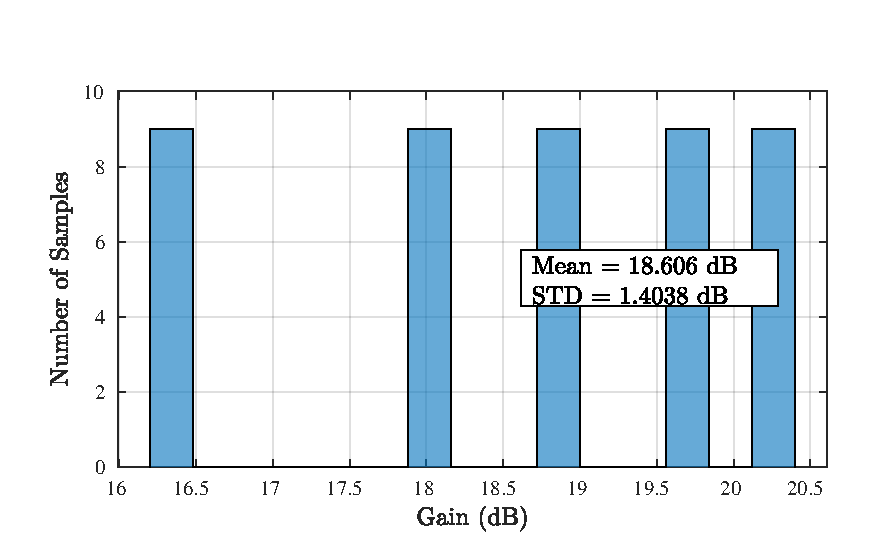
\includegraphics[scale=1]{Figures/Corners/Overall/Proc_Min/PDFs/Proc_Min_gain.pdf}
\caption{Histogram of System Gain due to Process Variation at $V_{bias}$=150mV}
\end{figure}

\begin{figure} [H]
\centering
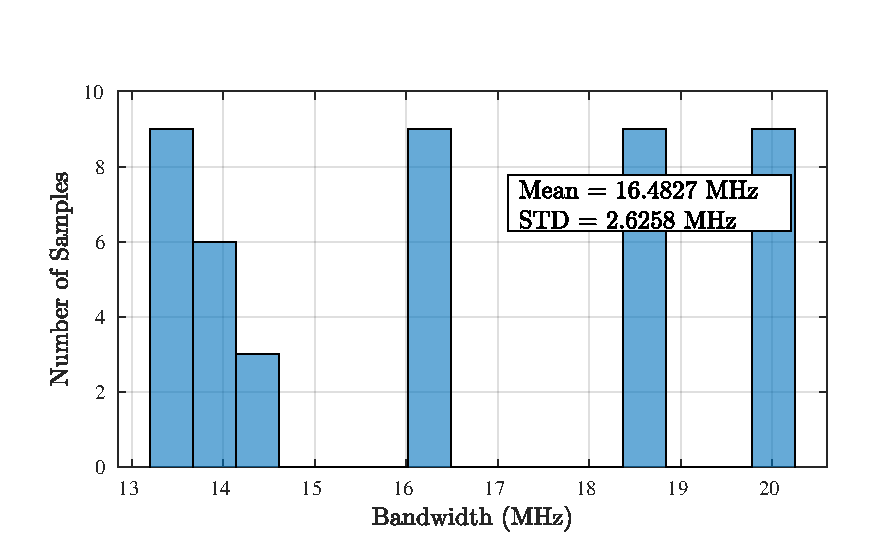
\includegraphics[scale=1]{Figures/Corners/Overall/Proc_Min/PDFs/Proc_Min_bw.pdf}
\caption{Histogram of System Bandwidth due to Process Variation at $V_{bias}$=150mV}
\end{figure}

\begin{figure} [H]
\centering
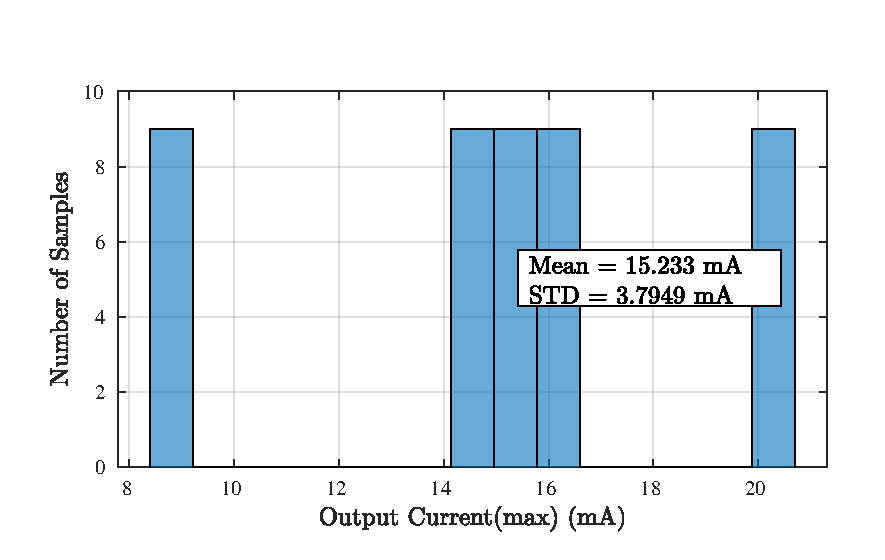
\includegraphics[scale=1]{Figures/Corners/Overall/Proc_Min/PDFs/Proc_Min_imax.pdf}
\caption{Histogram of Maximum Output Current due to Process Variation at $V_{bias}$=150mV}
\end{figure}

\begin{figure} [H]
\centering
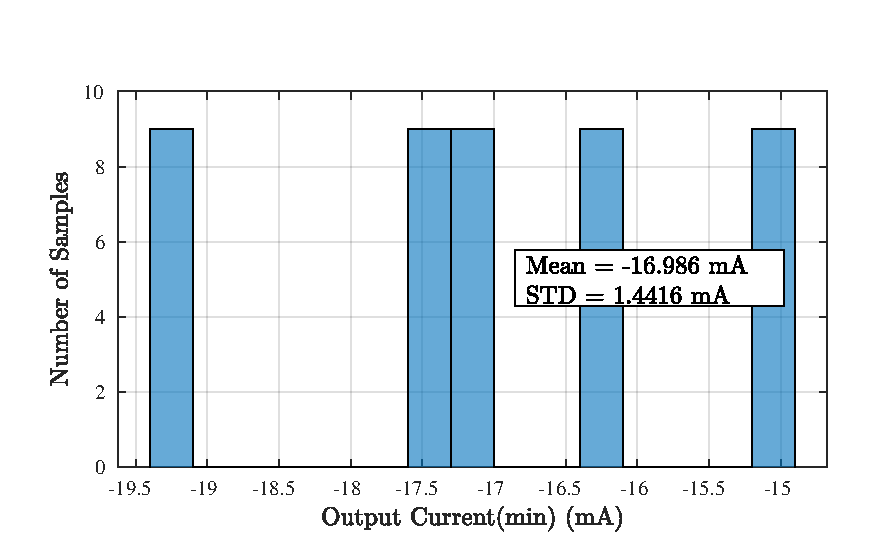
\includegraphics[scale=1]{Figures/Corners/Overall/Proc_Min/PDFs/Proc_Min_imin.pdf}
\caption{Histogram of Minimum Output Current due to Process Variation at $V_{bias}$=150mV}
\end{figure}

\subsubsection{Highest $V_{bias}$}
At the highest $V_{bias}$, the mean values of the parameters meet the requirements. At the worst corner, the positive peak of the output current slips to 20mA but the peak to peak current is still under the requirement. Since the spread is smaller for all parameters, none of them fail to meet the requirements.
\begin{figure} [H]
\centering
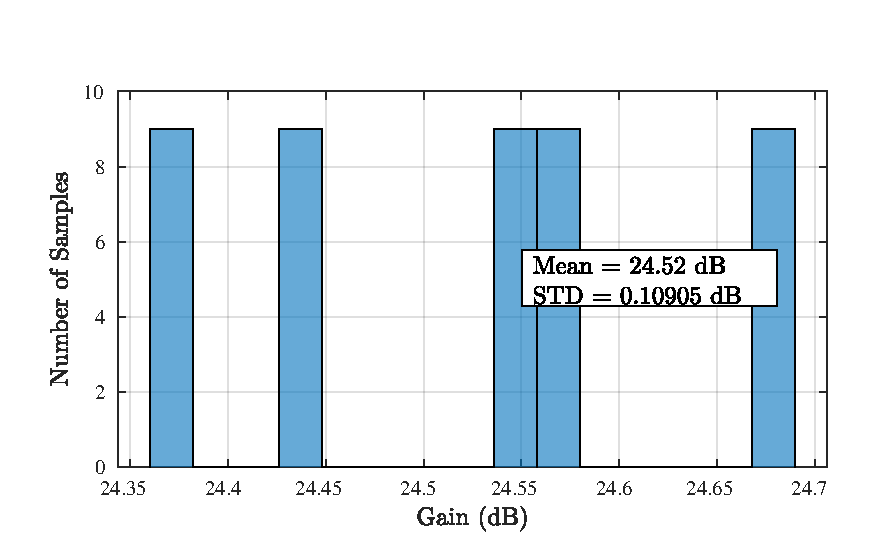
\includegraphics[scale=1]{Figures/Corners/Overall/Proc_Max/PDFs/Proc_Max_gain.pdf}
\caption{Histogram of System Gain due to Process Variation at $V_{bias}$=700mV}
\end{figure}

\begin{figure} [H]
\centering
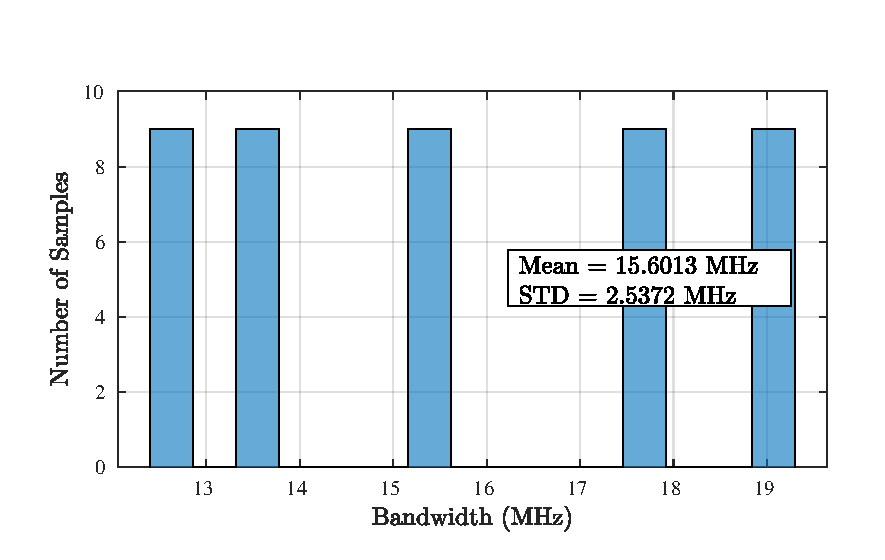
\includegraphics[scale=1]{Figures/Corners/Overall/Proc_Max/PDFs/Proc_Max_bw.pdf}
\caption{Histogram of System Bandwidth due to Process Variation at $V_{bias}$=700mV}
\end{figure}

\begin{figure} [H]
\centering
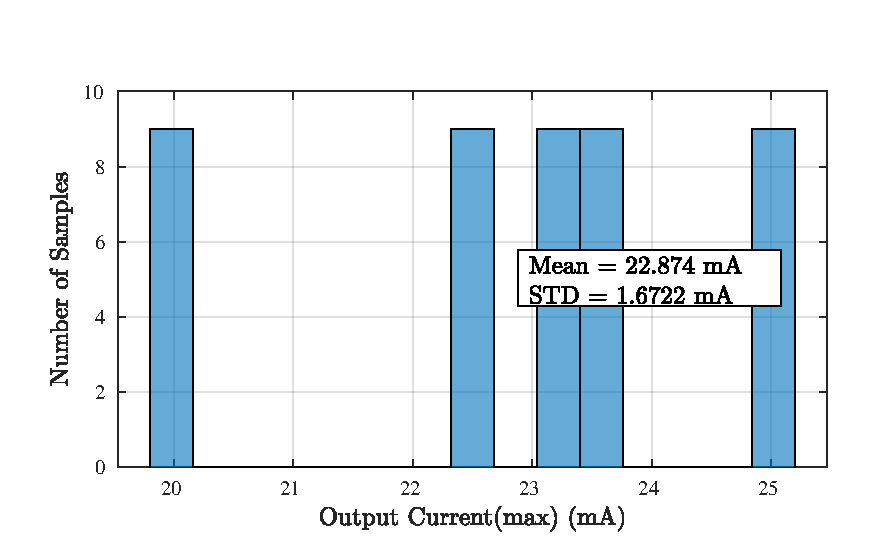
\includegraphics[scale=1]{Figures/Corners/Overall/Proc_Max/PDFs/Proc_Max_imax.pdf}
\caption{Histogram of Maximum Output Current due to Process Variation at $V_{bias}$=700mV}
\end{figure}

\begin{figure} [H]
\centering
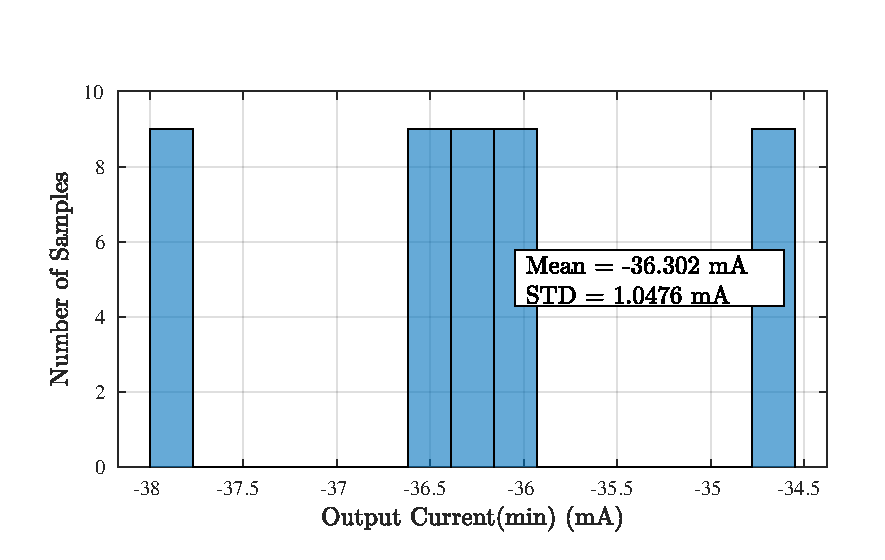
\includegraphics[scale=1]{Figures/Corners/Overall/Proc_Max/PDFs/Proc_Max_imin.pdf}
\caption{Histogram of Minimum Output Current due to Process Variation at $V_{bias}$=700mV}
\end{figure}

\section{Process and Supply Variation}

In addition to process variation, the system responds to power supply variations too. 3 different corners are obtained by evaluating the power supply with $\pm$10\% from the nominal value. Therefore, we get 3 corners for $V_{DD}$ - 2.5V, 2.25V, 2.75V and 3 corners for $V_{SS}$ - -2.5V, -2.25V, -2.75V. The total number of corners in this case are 405. And the results are discussed in the subsequent sections.

\subsubsection{Lowest $V_{bias}$}
Additional variation in power supply increases the spread in the histogram with samples for gain at 12dB and as high as 21dB. The mean values of all parameters are well within their specified range. But the positive peak output current value drops to a negative value for the worst case. The negative output current for the same case is at -10mA which makes the peak to peak current of 9mA, which is little far from what is required.

\begin{figure} [H]
\centering
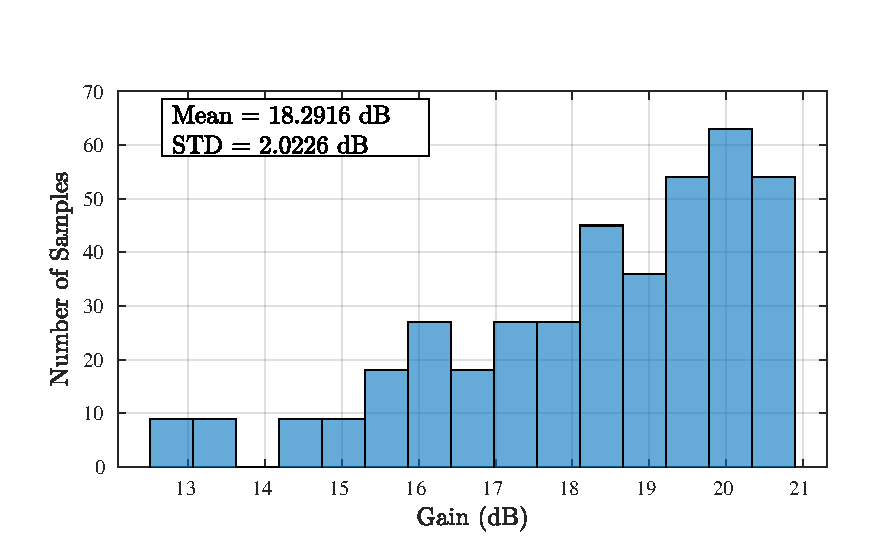
\includegraphics[scale=1]{Figures/Corners/Overall/PV_Min/PDFs/PV_Min_gain.pdf}
\caption{Histogram of System Gain due to Process and Supply Variation at $V_{bias}$=150mV}
\end{figure}

\begin{figure} [H]
\centering
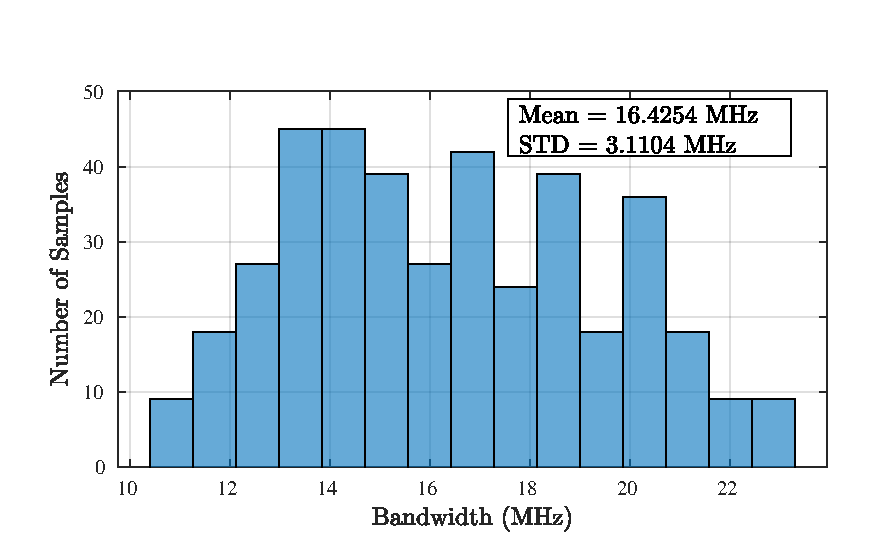
\includegraphics[scale=1]{Figures/Corners/Overall/PV_Min/PDFs/PV_Min_bw.pdf}
\caption{Histogram of System Bandwidth due to Process and Supply Variation at $V_{bias}$=150mV}
\end{figure}

\begin{figure} [H]
\centering
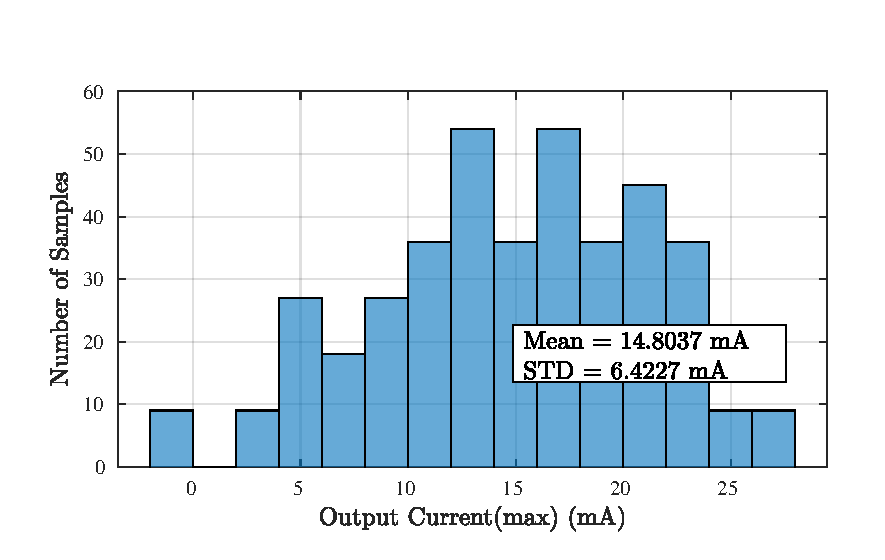
\includegraphics[scale=1]{Figures/Corners/Overall/PV_Min/PDFs/PV_Min_imax.pdf}
\caption{Histogram of Maximum Output Current due to Process and Supply Variation at $V_{bias}$=150mV}
\end{figure}

\begin{figure} [H]
\centering
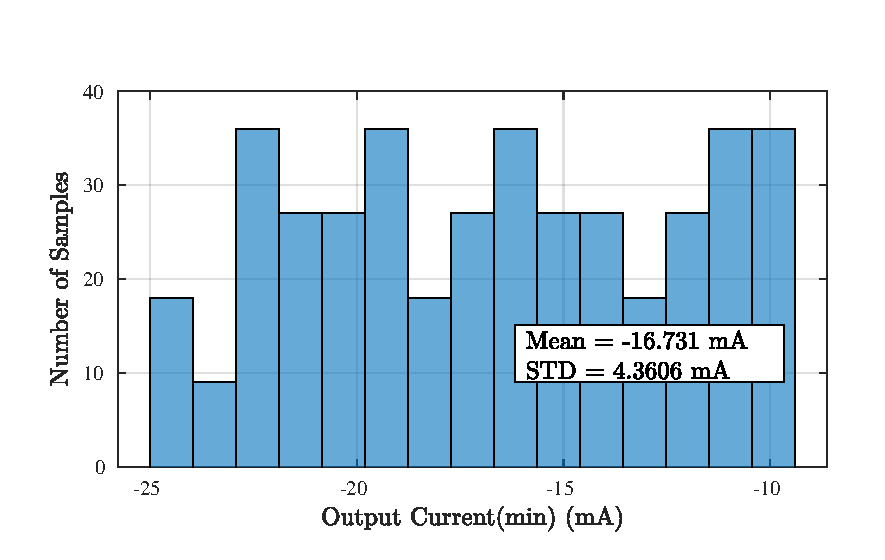
\includegraphics[scale=1]{Figures/Corners/Overall/PV_Min/PDFs/PV_Min_imin.pdf}
\caption{Histogram of Minimum Output Current due to Process and Supply Variation at $V_{bias}$=150mV}
\end{figure}

\begin{figure} [H]
\centering
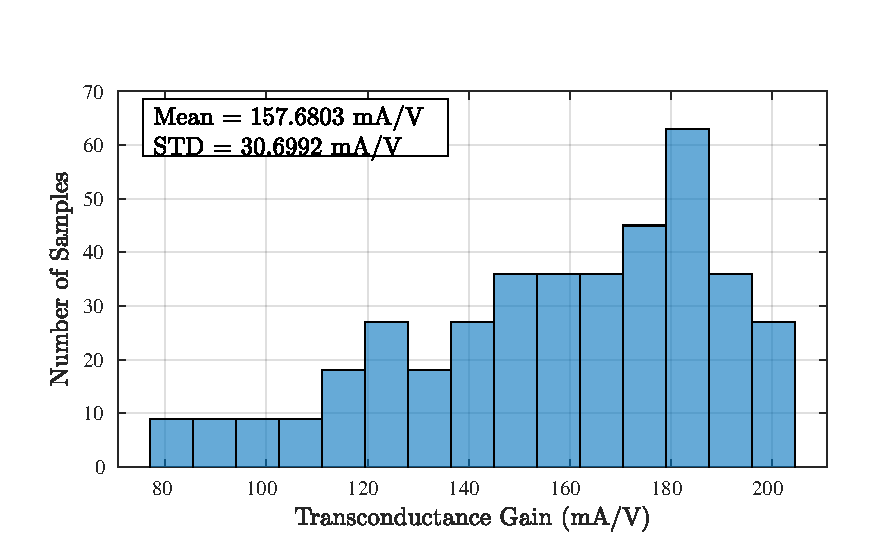
\includegraphics[scale=1]{Figures/Corners/Overall/PV_Min/PDFs/PV_Min_gm.pdf}
\caption{Histogram of Transconductance due to Process and Supply Variation at $V_{bias}$=150mV}
\end{figure}

\subsubsection{Highest $V_{bias}$}
The spread is wide for the bandwidth but even in the worst corner, the bandwidth is above 10MHz and the mean value being 15MHz. The spread for the gain is comparatively smaller with the mean value being 24.5dB and the standard deviation of 0.62dB. The slow corners are once again the worst case corners with the positive current peak dropping 16mA from a mean value of 22mA.
\begin{figure} [H]
\centering
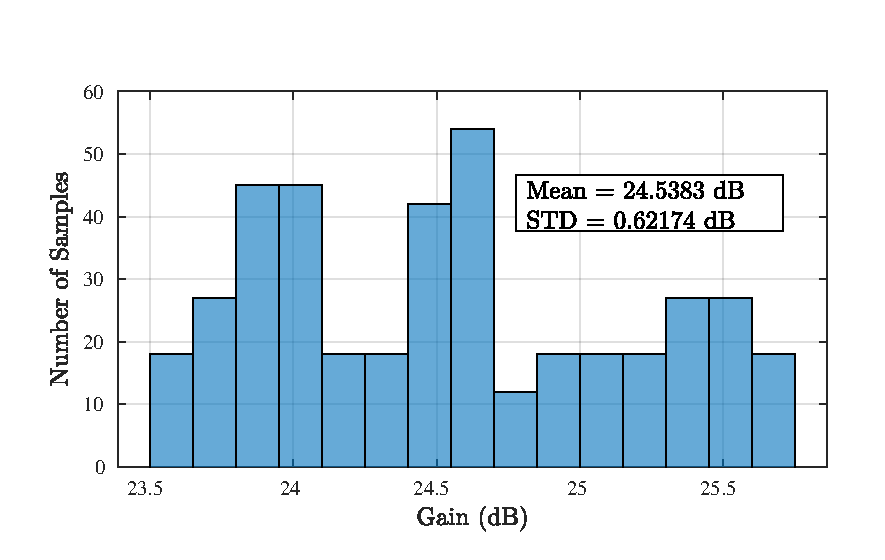
\includegraphics[scale=1]{Figures/Corners/Overall/PV_Max/PDFs/PV_Max_gain.pdf}
\caption{Histogram of System Gain due to Process and Supply Variation at $V_{bias}$=700mV}
\end{figure}

\begin{figure} [H]
\centering
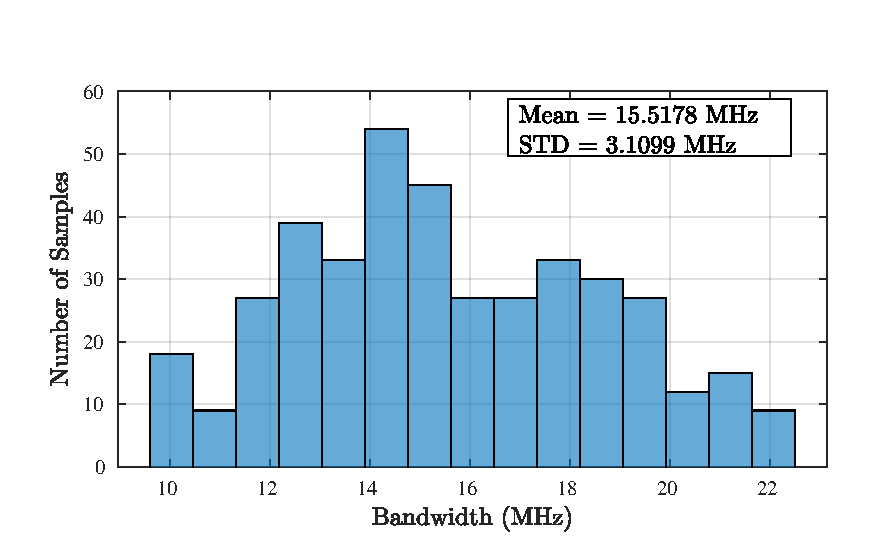
\includegraphics[scale=1]{Figures/Corners/Overall/PV_Max/PDFs/PV_Max_bw.pdf}
\caption{Histogram of System Bandwidth due to Process and Supply Variation at $V_{bias}$=700mV}
\end{figure}

\begin{figure} [H]
\centering
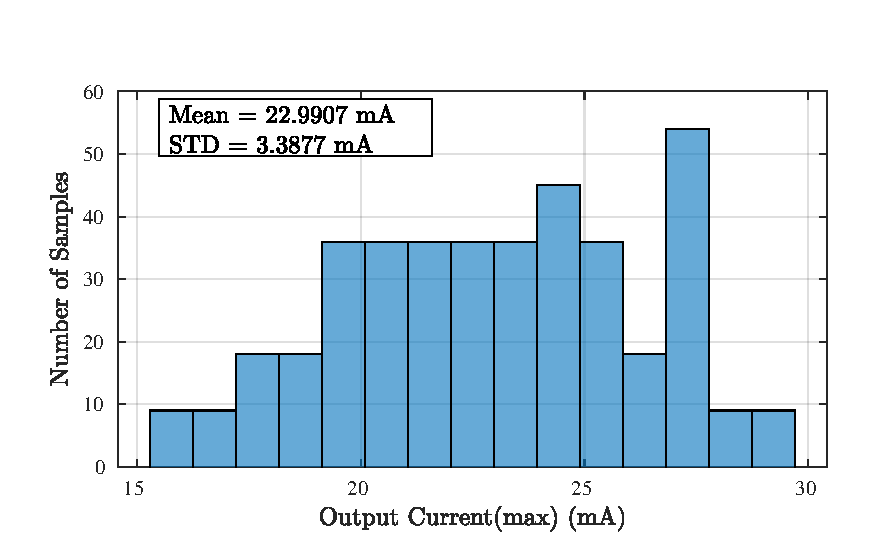
\includegraphics[scale=1]{Figures/Corners/Overall/PV_Max/PDFs/PV_Max_imax.pdf}
\caption{Histogram of Maximum Output Current due to Process and Supply Variation at $V_{bias}$=700mV}
\end{figure}

\begin{figure} [H]
\centering
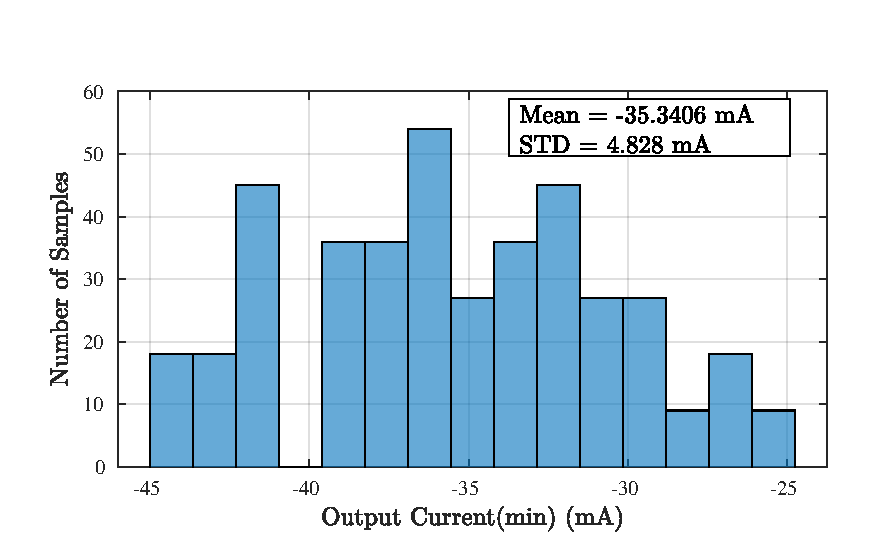
\includegraphics[scale=1]{Figures/Corners/Overall/PV_Max/PDFs/PV_Max_imin.pdf}
\caption{Histogram of Minimum Output Current due to Process and Supply Variation at $V_{bias}$=700mV}
\end{figure}

\begin{figure} [H]
\centering
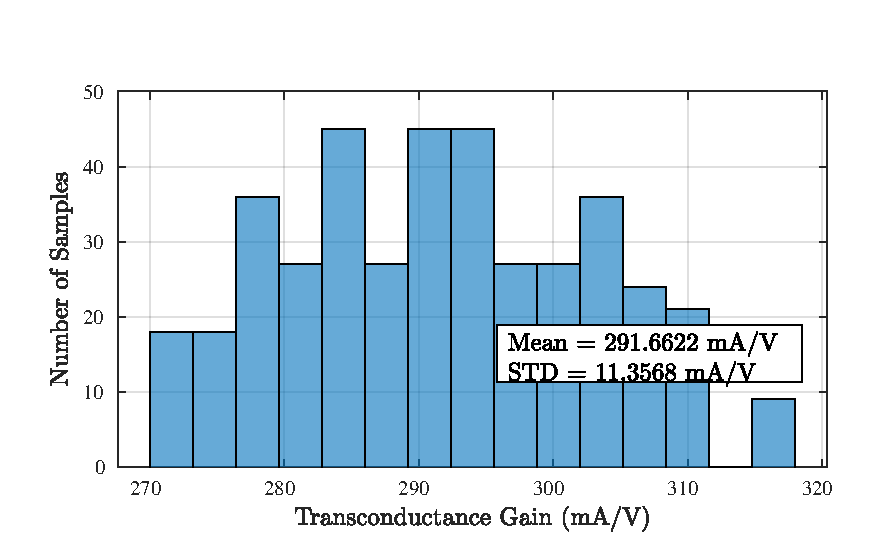
\includegraphics[scale=1]{Figures/Corners/Overall/PV_Max/PDFs/PV_Max_gm.pdf}
\caption{Histogram of Transconductance due to Process and Supply Variation at $V_{bias}$=700mV}
\end{figure}

\begin{figure} [H]
\centering
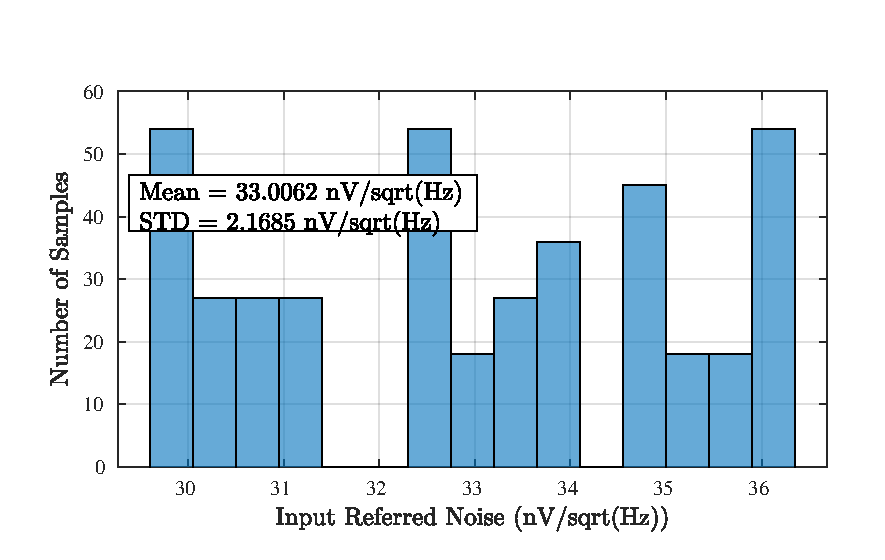
\includegraphics[scale=1]{Figures/Corners/Overall/PV_Max/PDFs/PV_Max_irn.pdf}
\caption{Histogram of Input Referred Noise due to Process and Supply Variation at $V_{bias}$=400mV}
\end{figure}

\section{Process, Voltage and Temperature (PVT) variation}

Another possible variation is seen in the temperature parameter. The PVT corner simulations are performed at the following corners:
\begin{itemize}
\item All Process corners mentioned in Section 4.6.1.
\item $\pm$10\% variations of $V_{DD}$ i.e., 2.5V, 2.25V, 2.75V and $V_{SS}$ i.e., -2.5V, -2.25V, -2.75V.
\item Three temperature conditions: -25$^0$C, 25$^0$C and 80$^0$C.
\end{itemize}

Therefore, there are 1215 corners in total. The results are provided in the subsequent sections.

\subsubsection{Lowest $V_{bias}$}
With all the variations included, it is observed that the worst case is caused by the supply variations and the temperature variation has lower effect than the suuply variation. The worst case corners are still affected by the voltage but with normal spread. The mean gain is 18.3dB with a standard deviation of 2.1dB. The bandwidth too has a wide spread like the gain histogram and at the worst case, it falls just a tad below 10MHz with the mean and standard deviation being 16MHz and 4MHz respectively. The HD2 and HD3 values are less than -30dBc even for worst cases. The PSRR however, at worst case, goes to a value beyond 160$\mu$A/V

\begin{figure} [H]
\centering
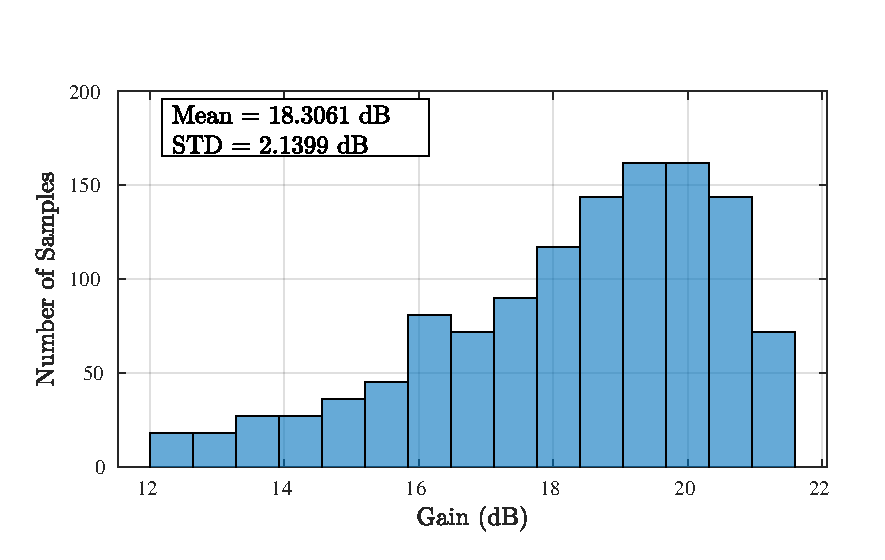
\includegraphics[scale=1]{Figures/Corners/Overall/PVT_Min/PDFs/PVT_Min_gain.pdf}
\caption{Histogram of System Gain due to PVT Variation at $V_{bias}$=150mV}
\end{figure}

\begin{figure} [H]
\centering
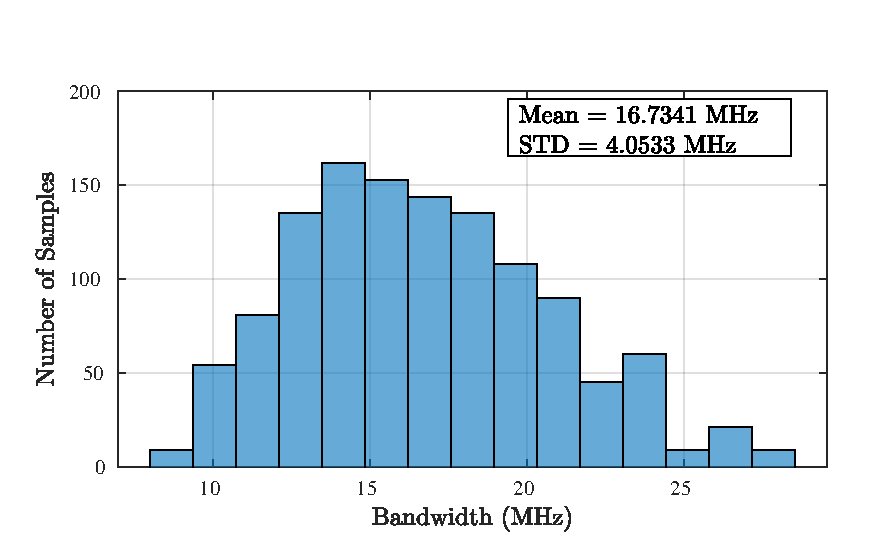
\includegraphics[scale=1]{Figures/Corners/Overall/PVT_Min/PDFs/PVT_Min_bw.pdf}
\caption{Histogram of System Bandwidth due to PVT Variation at $V_{bias}$=150mV}
\end{figure}

\begin{figure} [H]
\centering
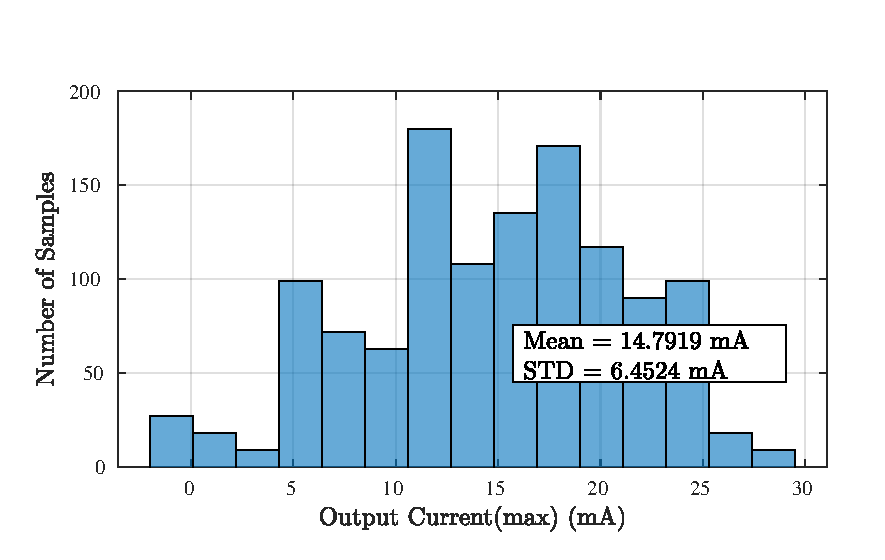
\includegraphics[scale=1]{Figures/Corners/Overall/PVT_Min/PDFs/PVT_Min_imax.pdf}
\caption{Histogram of Maximum Output Current due to PVT Variation at $V_{bias}$=150mV}
\end{figure}

\begin{figure} [H]
\centering
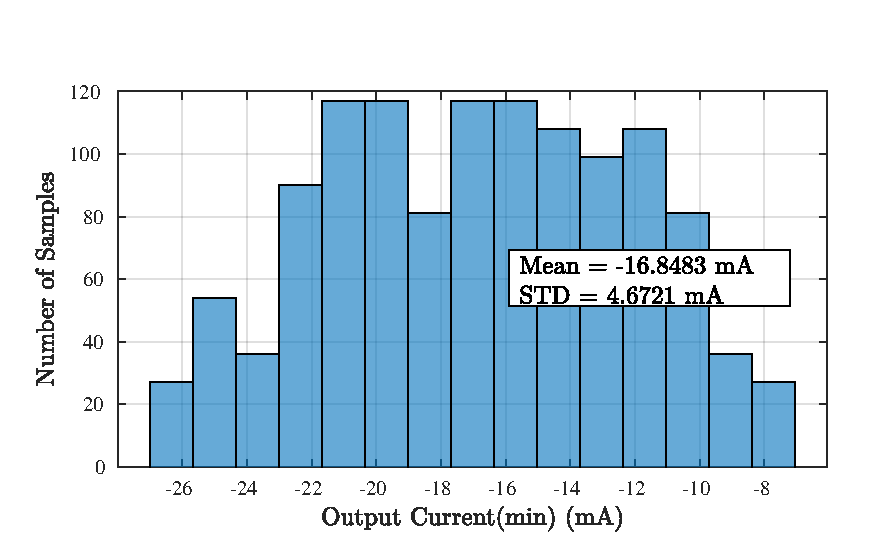
\includegraphics[scale=1]{Figures/Corners/Overall/PVT_Min/PDFs/PVT_Min_imin.pdf}
\caption{Histogram of Minimum Output Current due to PVT Variation at $V_{bias}$=150mV}
\end{figure}

\begin{figure} [H]
\centering
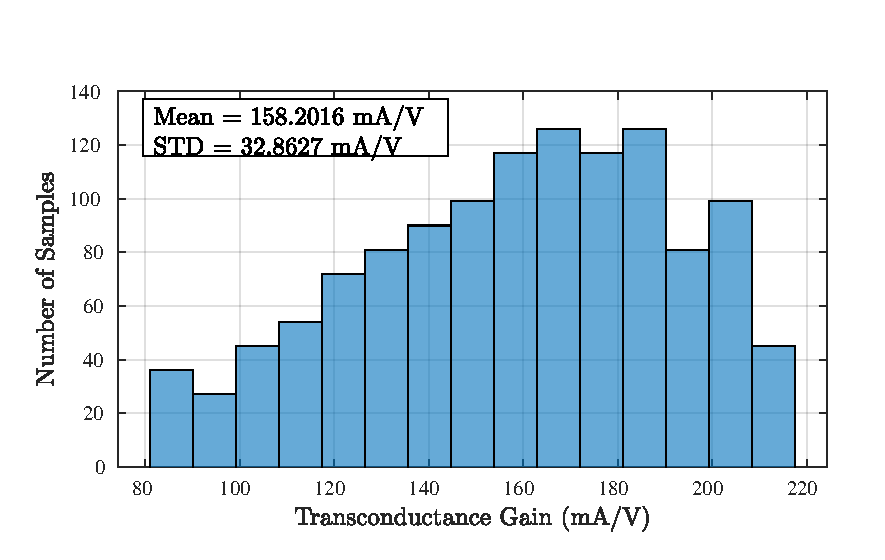
\includegraphics[scale=1]{Figures/Corners/Overall/PVT_Min/PDFs/PVT_Min_gm.pdf}
\caption{Histogram of Transconductance due to PVT Variation at $V_{bias}$=150mV}
\end{figure}

\begin{figure} [H]
\centering
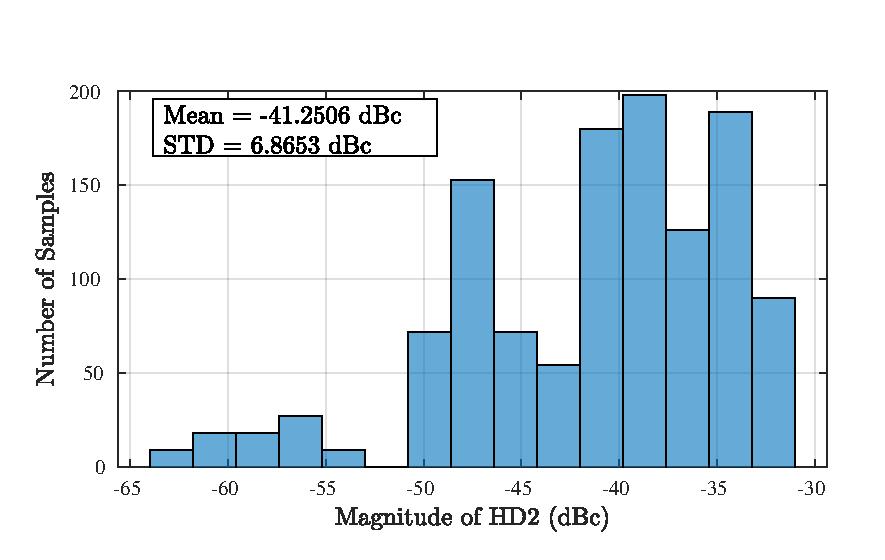
\includegraphics[scale=1]{Figures/Corners/Overall/PVT_Min/PDFs/PVT_Min_hd2.pdf}
\caption{Histogram of HD2 due to PVT Variation at $V_{bias}$=150mV}
\end{figure}

\begin{figure} [H]
\centering
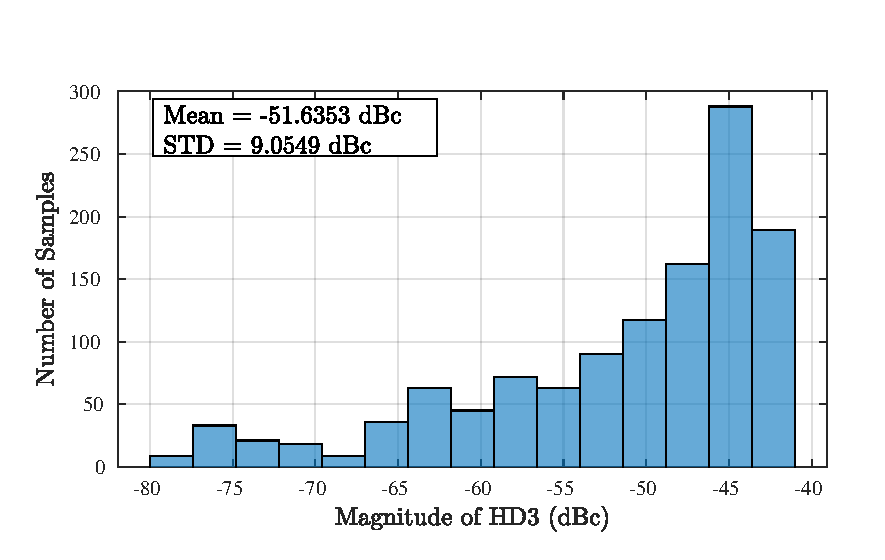
\includegraphics[scale=1]{Figures/Corners/Overall/PVT_Min/PDFs/PVT_Min_hd3.pdf}
\caption{Histogram of HD3 due to PVT at $V_{bias}$=150mV}
\end{figure}

\begin{figure} [H]
\centering
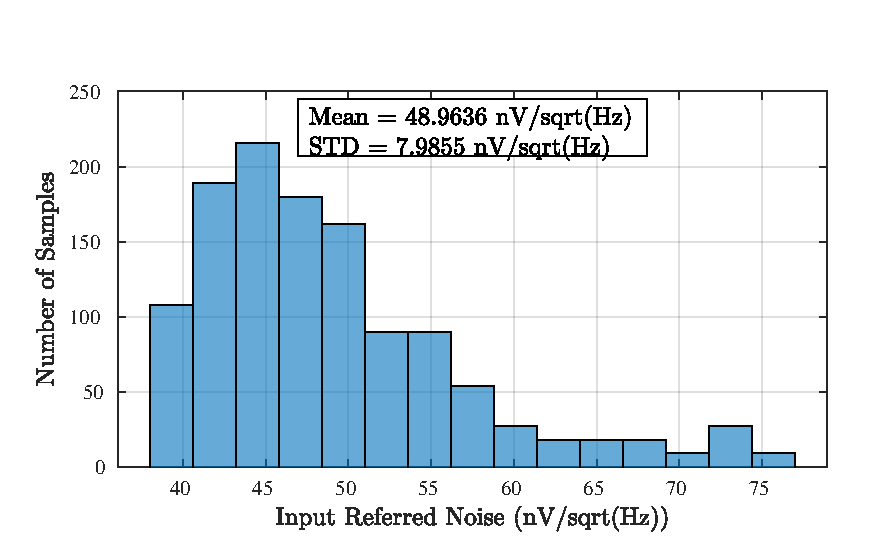
\includegraphics[scale=1]{Figures/Corners/Overall/PVT_Min/PDFs/PVT_Min_irn.pdf}
\caption{Histogram of Input Referred Noise due to PVT Variation at $V_{bias}$=150mV}
\end{figure}

\begin{figure} [H]
\centering
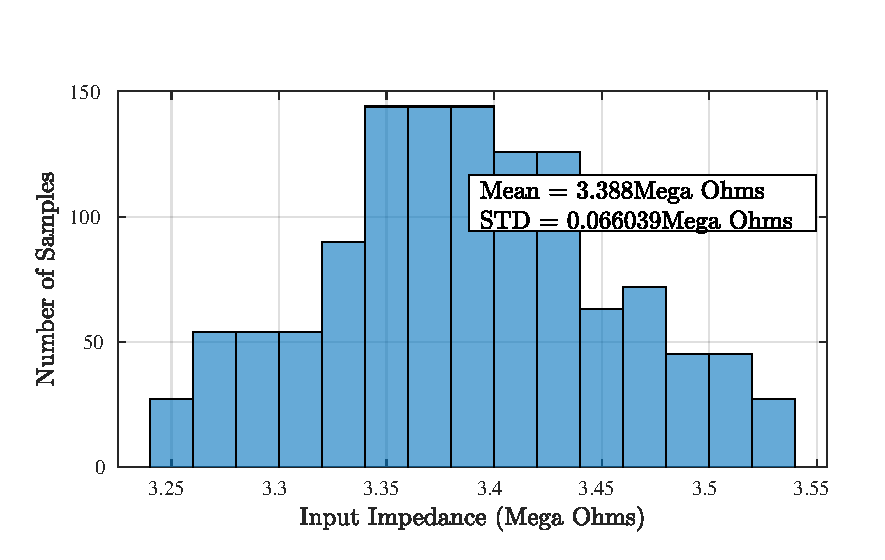
\includegraphics[scale=1]{Figures/Corners/Overall/PVT_Min/PDFs/PVT_Min_zin.pdf}
\caption{Histogram of Input Impedance due to PVT Variation at $V_{bias}$=150mV}
\end{figure}

\begin{figure} [H]
\centering
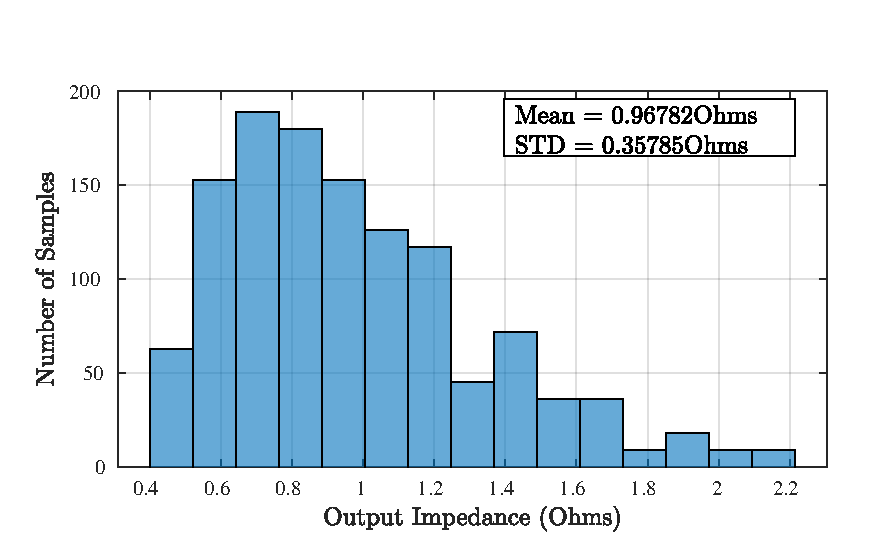
\includegraphics[scale=1]{Figures/Corners/Overall/PVT_Min/PDFs/PVT_Min_zout.pdf}
\caption{Histogram of Output Impedance due to PVT Variation at $V_{bias}$=150mV}
\end{figure}

\begin{figure} [H]
\centering
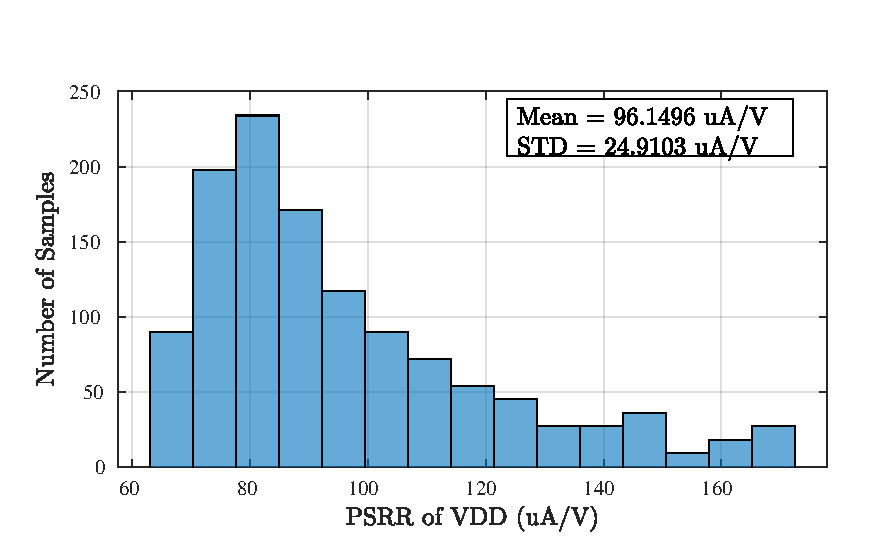
\includegraphics[scale=1]{Figures/Corners/Overall/PVT_Min/PDFs/PVT_Min_psrrp.pdf}
\caption{Histogram of PSRR($V_{DD}$) due to PVT Variation at $V_{bias}$=150mV}
\end{figure}

\begin{figure} [H]
\centering
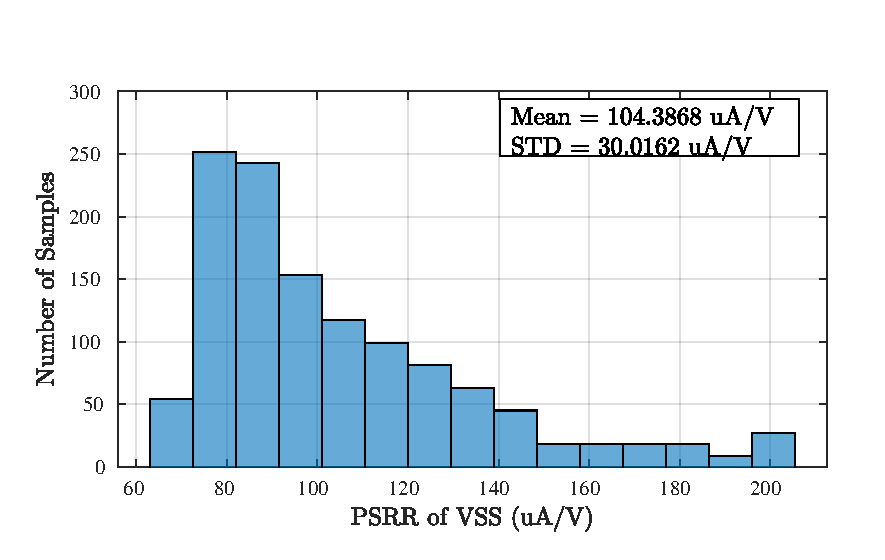
\includegraphics[scale=1]{Figures/Corners/Overall/PVT_Min/PDFs/PVT_Min_psrrn.pdf}
\caption{Histogram of PSRR($V_{SS}$) due to PVT Variation at $V_{bias}$=150mV}
\end{figure}

\subsubsection{Highest $V_{bias}$}
For the highest $V_{bias}$, the mean gain is around 24dB with a standard deviation of 0.7dB. The spread for the gain histogram is comparatively narrower in comparison to the lowest $V_{bias}$. Once again the bandwidth just falls short of 10MHz for the worst case corner. The mean values of the currents are 23mA and -35mA. But at the worst case corner, the peak-to-peak current is as low as 40mA. The mean values of HD2 and HD3 are below -30dBc but they rise above the -30dBc mark for slow corners. The input referred noise spread is much smaller for highest $V_{bias}$ with a mean value of 32.985nV/$\sqrt{Hz}$.

\begin{figure} [H]
\centering
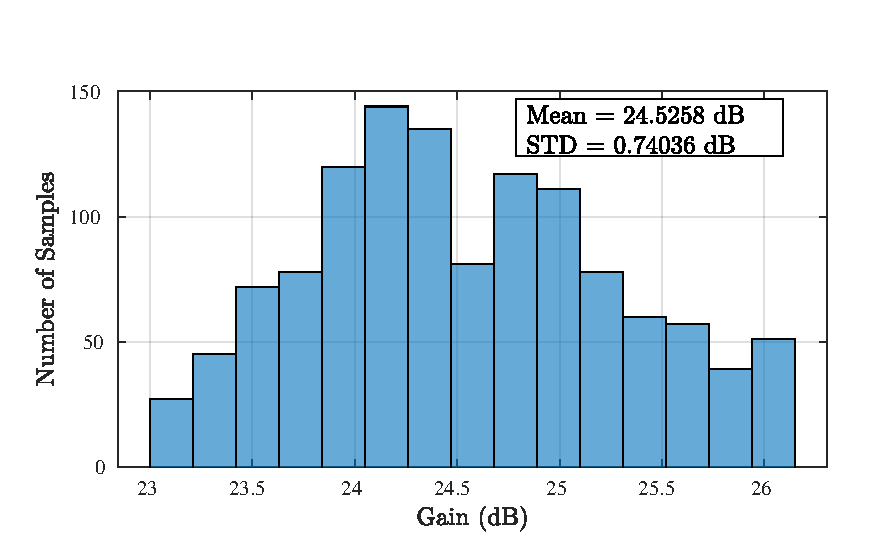
\includegraphics[scale=1]{Figures/Corners/Overall/PVT_Max/PDFs/PVT_Max_gain.pdf}
\caption{Histogram of System Gain due to PVT Variation at $V_{bias}$=700mV}
\end{figure}

\begin{figure} [H]
\centering
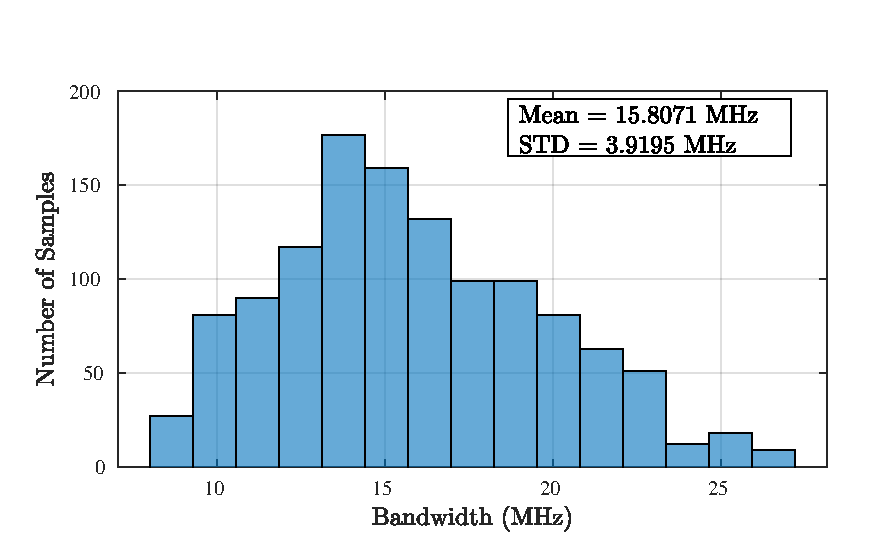
\includegraphics[scale=1]{Figures/Corners/Overall/PVT_Max/PDFs/PVT_Max_bw.pdf}
\caption{Histogram of System Bandwidth due to PVT Variation at $V_{bias}$=700mV}
\end{figure}

\begin{figure} [H]
\centering
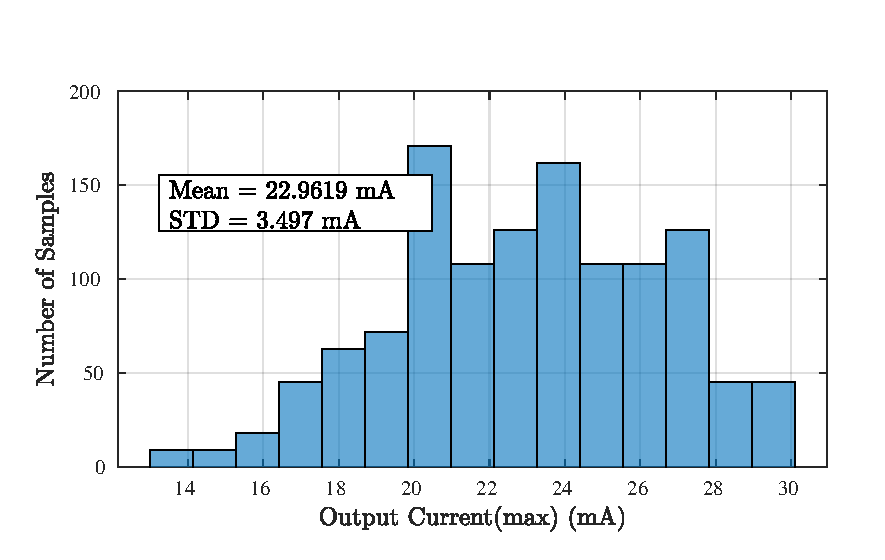
\includegraphics[scale=1]{Figures/Corners/Overall/PVT_Max/PDFs/PVT_Max_imax.pdf}
\caption{Histogram of Maximum Output Current due to PVT Variation at $V_{bias}$=700mV}
\end{figure}

\begin{figure} [H]
\centering
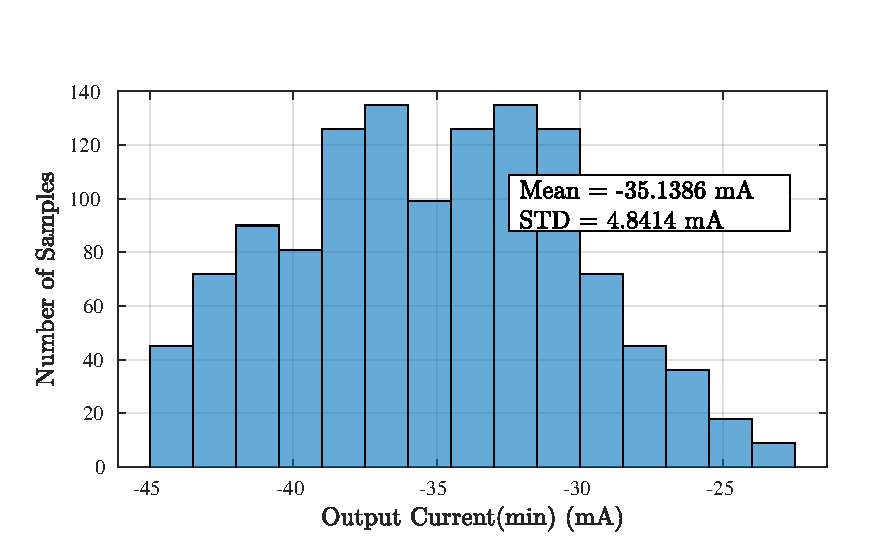
\includegraphics[scale=1]{Figures/Corners/Overall/PVT_Max/PDFs/PVT_Max_imin.pdf}
\caption{Histogram of Minimum Output Current due to PVT Variation at $V_{bias}$=700mV}
\end{figure}

\begin{figure} [H]
\centering
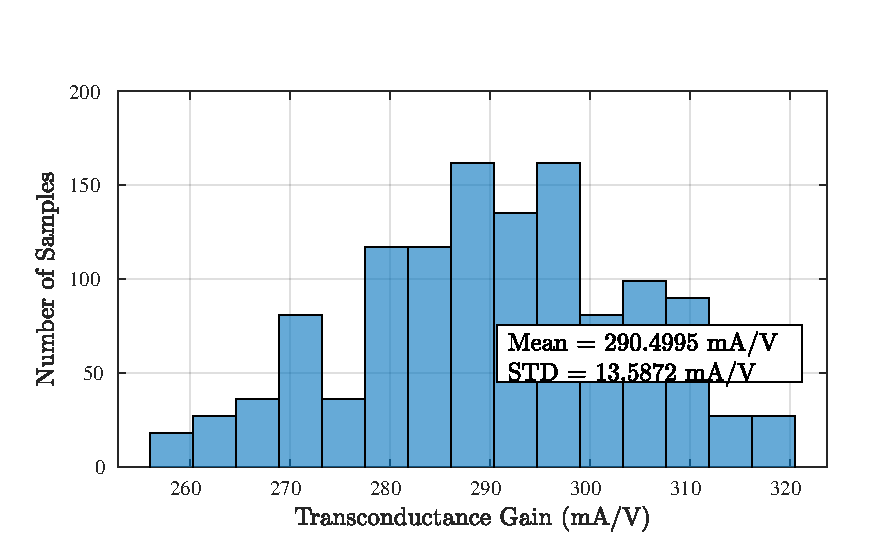
\includegraphics[scale=1]{Figures/Corners/Overall/PVT_Max/PDFs/PVT_Max_gm.pdf}
\caption{Histogram of Transconductance due to PVT Variation at $V_{bias}$=700mV}
\end{figure}

\begin{figure} [H]
\centering
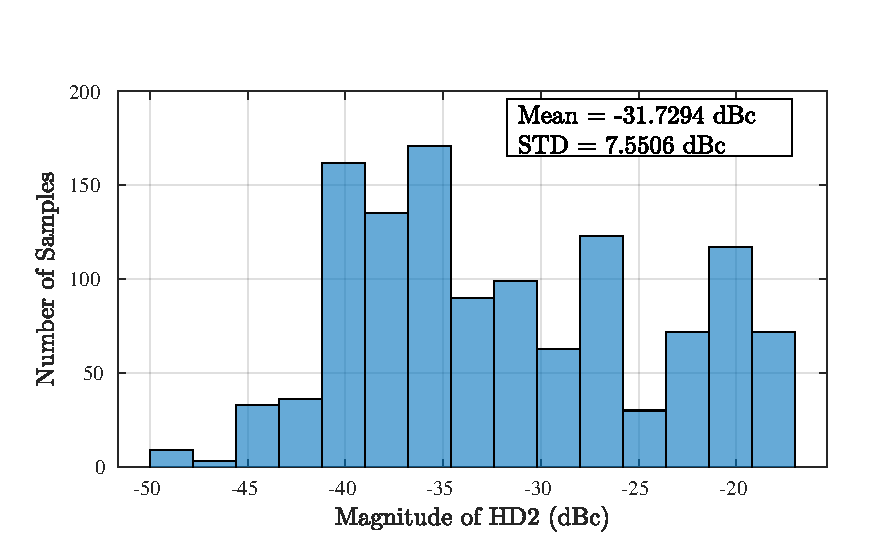
\includegraphics[scale=1]{Figures/Corners/Overall/PVT_Max/PDFs/PVT_Max_hd2.pdf}
\caption{Histogram of HD2 due to PVT Variation at $V_{bias}$=700mV}
\end{figure}

\begin{figure} [H]
\centering
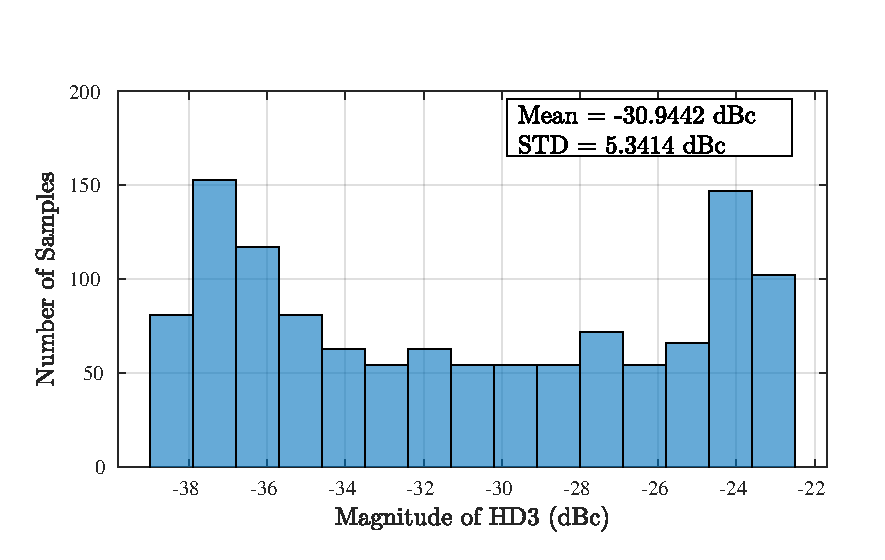
\includegraphics[scale=1]{Figures/Corners/Overall/PVT_Max/PDFs/PVT_Max_hd3.pdf}
\caption{Histogram of HD3 due to PVT Variation at $V_{bias}$=700mV}
\end{figure}

\begin{figure} [H]
\centering
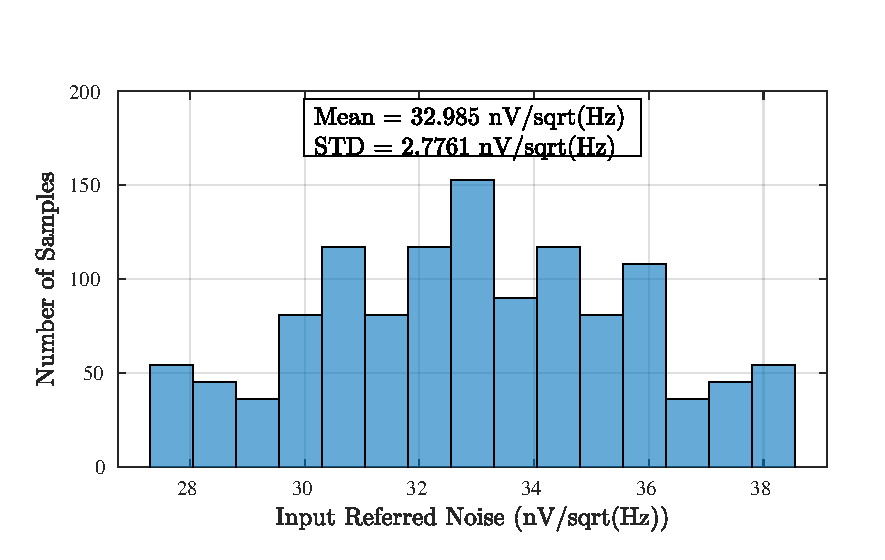
\includegraphics[scale=1]{Figures/Corners/Overall/PVT_Max/PDFs/PVT_Max_irn.pdf}
\caption{Histogram of Input Referred Noise due to PVT Variation at $V_{bias}$=400mV}
\end{figure}

\begin{figure} [H]
\centering
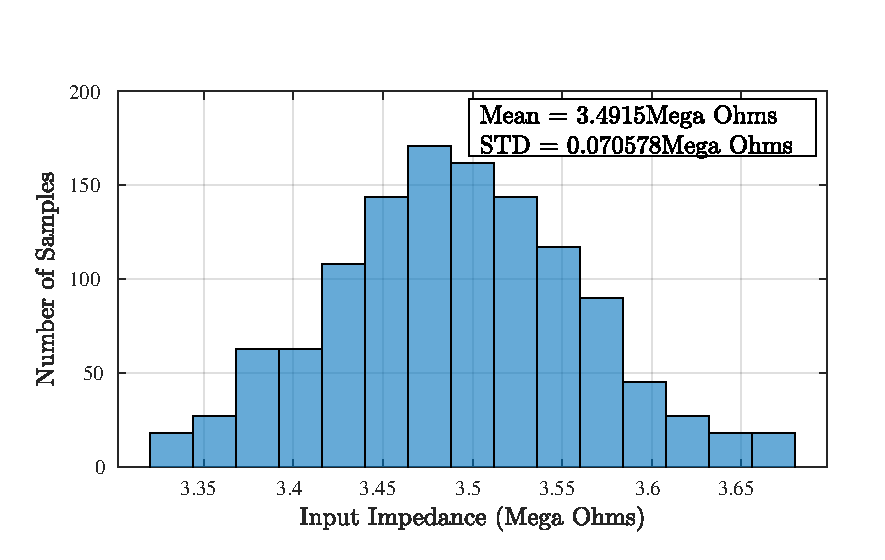
\includegraphics[scale=1]{Figures/Corners/Overall/PVT_Max/PDFs/PVT_Max_zin.pdf}
\caption{Histogram of Input Impedance due to PVT Variation at $V_{bias}$=700mV}
\end{figure}

\begin{figure} [H]
\centering
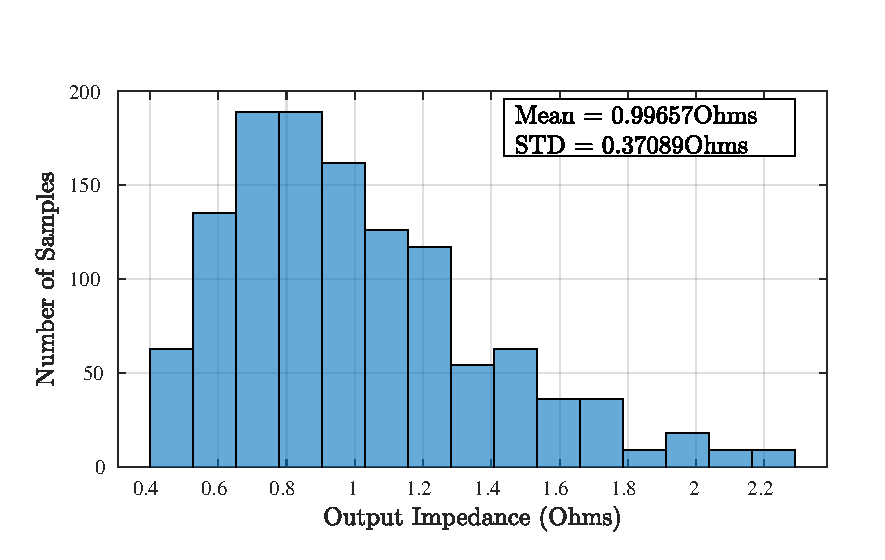
\includegraphics[scale=1]{Figures/Corners/Overall/PVT_Max/PDFs/PVT_Max_zout.pdf}
\caption{Histogram of Output Impedance due to Process and Supply Variation at $V_{bias}$=700mV}
\end{figure}

\begin{figure} [H]
\centering
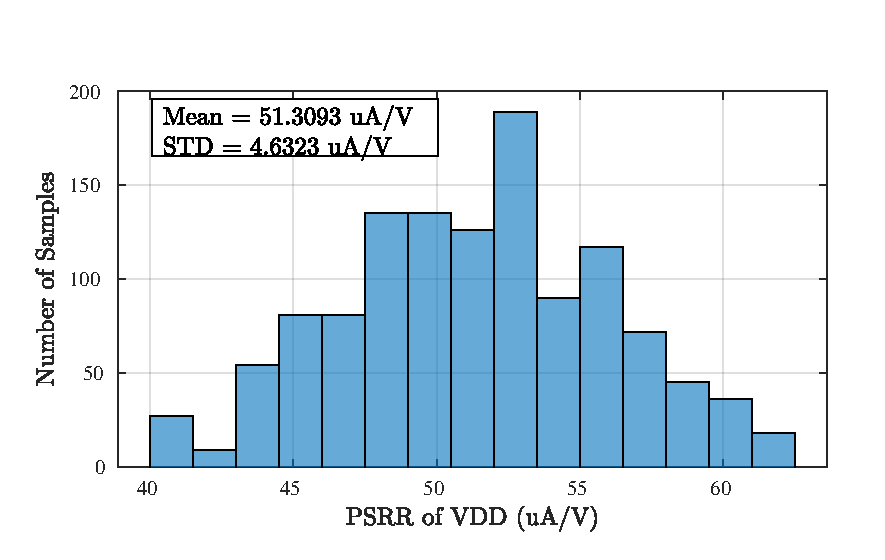
\includegraphics[scale=1]{Figures/Corners/Overall/PVT_Max/PDFs/PVT_Max_psrrp.pdf}
\caption{Histogram of PSRR($V_{DD}$) due to PVT Variation at $V_{bias}$=700mV}
\end{figure}

\begin{figure} [H]
\centering
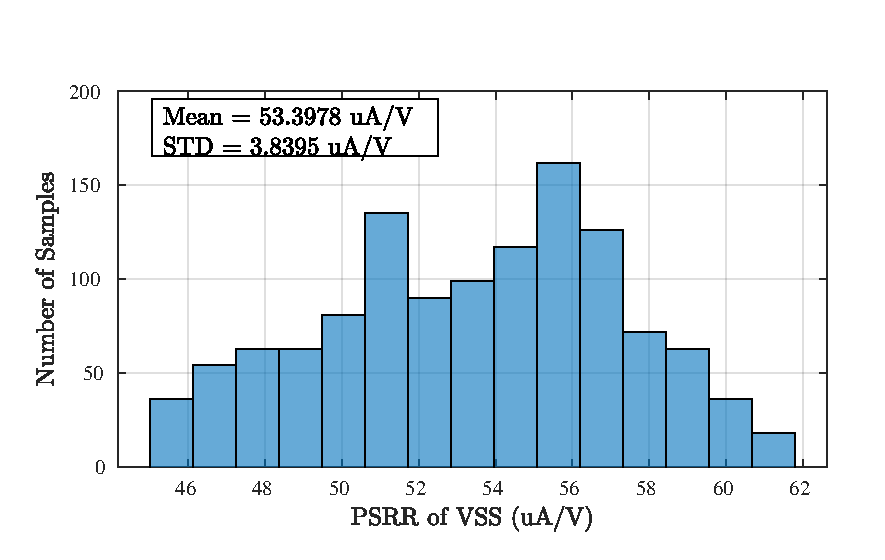
\includegraphics[scale=1]{Figures/Corners/Overall/PVT_Max/PDFs/PVT_Max_psrrn.pdf}
\caption{Histogram of PSRR($V_{SS}$) due to PVT Variation at $V_{bias}$=700mV}
\end{figure}

\vfill
\clearpage
\section{Summary of PVT Corner Analysis}